\section{背景知识}

本章介绍有关AdaptiveLLM的背景知识。由于AdaptiveLLM主要面向LLM推理过程中产生的KV Cache张量进行优化,因此本章将在第一节阐明KV Cache在LLM推理任务中的功能;第二节论述两个面向KV Cache的常见优化方向;第三节列举两个传统工作中针对KV Cache的张量优化技术。

\subsection{KV Cache的提出}

LLM推理任务以token作为输入与输出的基本单位。对于生成式推理任务,每次前向传播计算仅生成一个新token。一般来说,其包含两个阶段:prefill阶段读取用户输入的token序列,生成第一个token;decode阶段分为多步进行,依次生成后续token,直至得到终止token。在推理过程中,每个token拥有一个key-value张量对,为自注意力机制下的编码结果。\par

在decode阶段中,每个token的计算均依赖于前序token的key值和value值。如果每次计算前都重新调用自注意力机制来获取前序token的key-value张量,则会产生大量不必要的时间开销。主流LLM推理服务\cite{Swapping, vLLM, ORCA, SpecInfer}框架普遍采用KV Cache数据结构来保存这些token的key-value张量,方便后续token的生成,避免重复计算,其工作原理如图\ref{Fig:KV Cache的功能示意图}所示。

\begin{figure}[!htbp]
  \renewcommand{\arraystretch}{1}
  \centering
  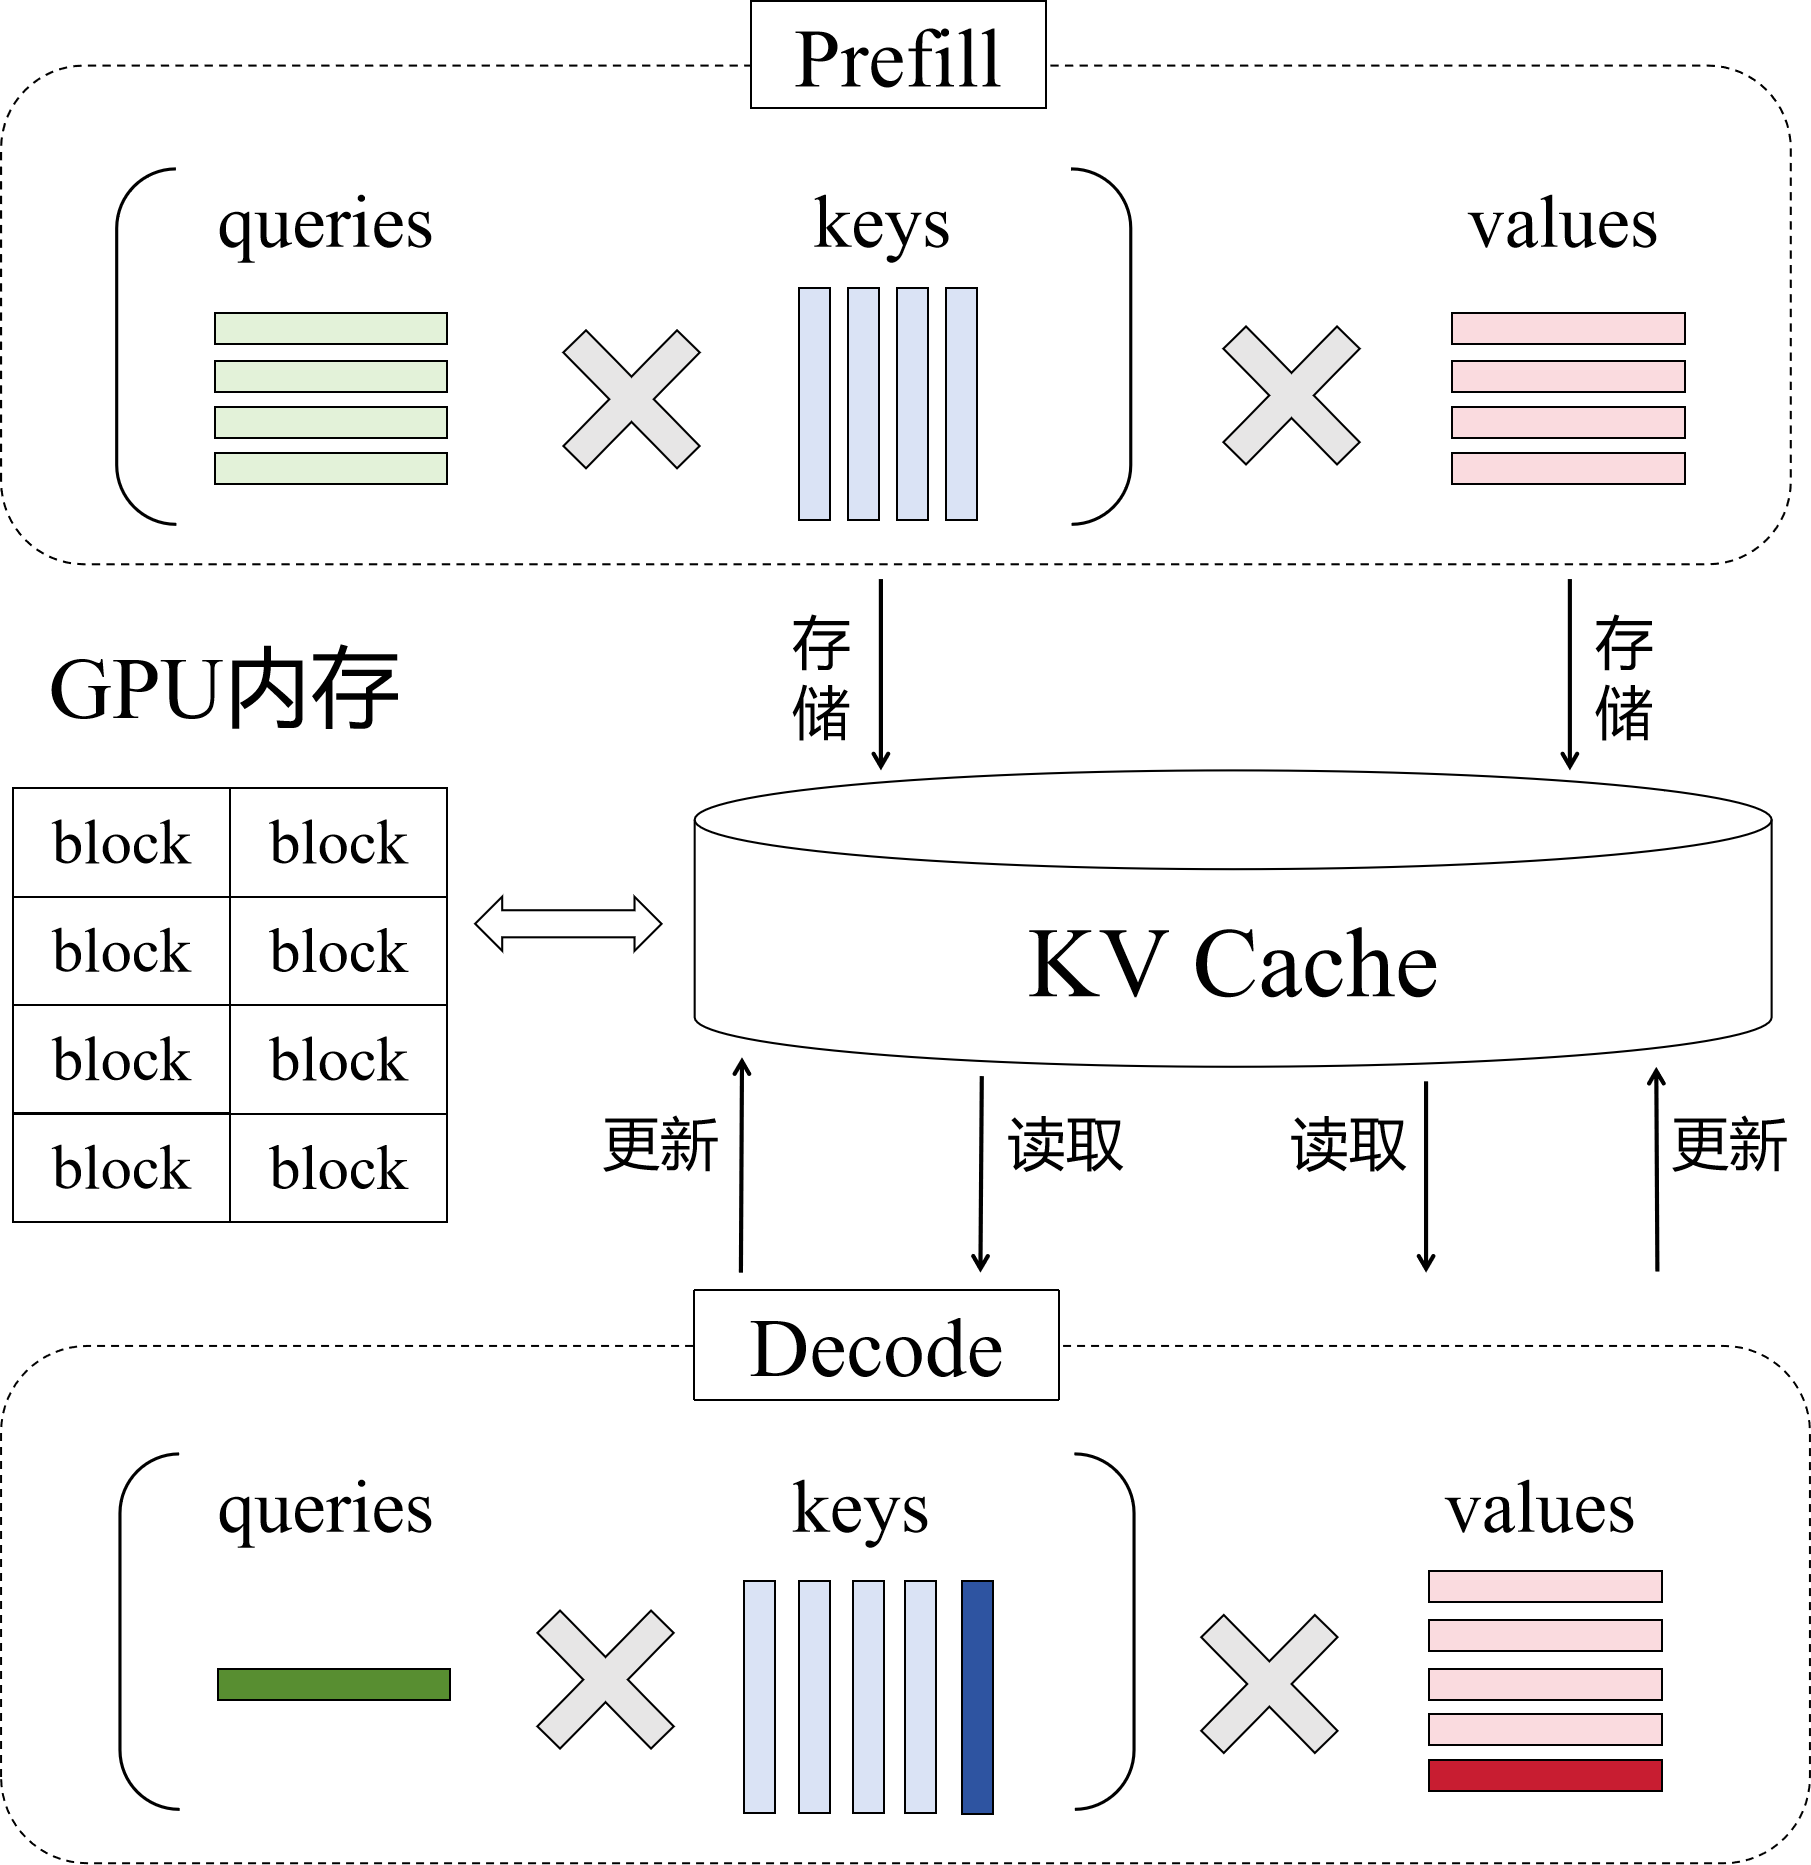
\includegraphics[width=0.9\linewidth]
  {KV Cache的功能示意图.png}
  \caption{KV Cache的功能示意图}
  \label{Fig:KV Cache的功能示意图}
\end{figure}

然而,随着后续token的不断生成,KV Cache迅速扩展,产生推理内存瓶颈。例如,在OPT-13B模型中,对于一个长度为100的用户请求,其KV Cache能够占用39.1MB的内存空间。有限的GPU内存将批处理大小限制在较低水平,阻碍推理并发度的进一步提升,进而限制吞吐率。\par

不同于LLM的参数张量,KV Cache在对应用户请求推理完毕后丢弃,其内存占用量大、动态性高,拥有较大的优化空间,因此AdaptiveLLM的内存优化策略将针对KV Cache实现。

\subsection{KV Cache的优化瓶颈}

KV Cache的引入方便了计算过程,却带来一些挑战,使得LLM推理性能的提升无法达到预期水平。下面介绍两个被人们所广泛讨论和研究的问题。

\subsubsection{内存利用率问题}

在传统LLM推理服务框架\cite{Swapping}中,内存管理器按照用户定义的序列长度上限,为每个请求设置一块固定大小的GPU内存来存储KV Cache。但用户请求长度的差异性导致内碎片的大量产生。为了解决该问题,部分LLM推理框架\cite{Output-Length-Prediction}能够基于历史信息来预测输出长度,并按照预测值分配内存。然而,预测误差会导致输出截断,且旧请求的完成与新请求的加入使得内存中产生很多外碎片。随着新请求的不断到来,内碎片与外碎片在内存中积累,严重影响了内存空间的高效使用。基于这些问题,vLLM框架\cite{vLLM}引入了Paged Attention机制,基于OS页式内存管理思想,将GPU内存划分成块,并通过维护块表来支持KV Cache在内存空间中的不连续存储。该机制基本消除了内碎片和外碎片现象,大大提升内存利用率。

\subsubsection{通信开销问题}

为了攻克推理内存瓶颈,传统框架引入了张量交换技术\cite{Swapping, vLLM, LightLLM},将暂时不会使用的KV Cache传输至CPU中,在计算需要时重新传输至GPU中。然而,CPU-GPU间有限的PCIe带宽使得换出和换入过程产生不可忽略的通信开销,限制吞吐率,降低推理性能。部分研究提出\cite{Recomputation},当张量交换带来的开销超过重新调用自注意力机制的开销时,应选择后者来获取所有前序token的key-value张量,也称张量重算。具体来说,内存管理器放弃张量的换出和换入过程,在用户请求被调度时执行一次prefill阶段来代替原本应该执行的decode阶段。重算与交换的联合使用缓解了通信开销问题,然而,当GPU内存不足时,如何在二者中进行选择成为了新的困境。AdaptiveLLM针对此问题设计了基于开销感知的内存优化策略,能够预测二者的开销,并选择开销小的过程执行。

\subsection{针对KV Cache的张量优化技术}

在LLM推理服务过程中,传统的张量优化(也称抢占)技术有三种:张量交换、张量重算和张量压缩\cite{Swapping}。AdaptiveLLM实现了张量交换与张量重算。而张量压缩目前还未能实现,将在本文第五章介绍。

\subsubsection{张量交换}

服务器拥有GPU-CPU-磁盘三级存储结构。GPU位于三级存储中的最上层,其计算速率快,并行度高,但存储空间有限,而CPU和磁盘的存储空间相对较大。为了提升服务器的实时吞吐率,LLM推理服务框架一般采用批处理的方式执行用户请求。随着批处理大小的增加或模型参数量的扩展,运行时需要保存的张量会超出GPU的内存限制。当检测到GPU内存占用峰值达到较高水平时,需要开启张量交换功能,将一部分需要保存,而暂时用不到的张量换出到CPU甚至磁盘中,在计算需要时重新换入GPU中。综上所述,张量交换包括换出与换入两个阶段,有两次数据传输过程。

\subsubsection{张量重算}

在抢占式用户请求调度系统中,当某个请求获得执行权时,会检查之前的计算结果是否保存在GPU中,如果不在,则需要重新获取这部分计算结果。此时可以无需将之前存储的计算结果(如果有)从CPU或磁盘中换入到GPU中,而仅仅对它们进行重新计算。对于执行LLM推理任务的用户请求而言,这些key-value张量在初次生成时经历了多次前向传播,而在重算过程中仅需调用自注意力机制即可得到,因此张量重算的开销远远小于token序列初次生成时的开销,不会导致计算量的爆炸式增长。